\documentclass[10pt]{article}
\usepackage{xr-hyper}
\usepackage{balance,times}
\usepackage{xcolor,microtype,enumitem,nth,,titlesec}
\usepackage[normalem]{ulem}
\usepackage{url,graphicx}
\usepackage[citestyle=authoryear-icomp,backend=bibtex]{biblatex}
\usepackage[pdflang={en-US},pdftex]{hyperref}
\usepackage{wrapfig,fancyhdr}
\usepackage[all]{hypcap}  % Fixes bug in hyperref caption linking
\usepackage[utf8]{inputenc} % for a UTF8 editor only

\usepackage[en-US]{datetime2}
\DTMsettimestyle{default}
\DTMsetup{showseconds=true}

% \usepackage{caption,setspace}
\bibliography{references}
\usepackage[margin=1in]{geometry}
% \pagestyle{fancy}
\titlespacing*{\section}{0.0ex}{2ex plus .3ex}{1ex plus .3ex}


\lhead{} % controls the left corner of the header
% \chead{} % controls the center of the header
\rhead{Ali Alkhatib \& Jeff Nagy} % controls the right corner of the header
\lfoot{} % controls the left corner of the footer
\lfoot{last updated \DTMcurrenttime~\today} % controls the left corner of the footer
\cfoot{} % controls the center of the footer
\rfoot{} % controls the right corner of the footer
% \rfoot{Page~\thepage} % controls the right corner of the footer
\renewcommand{\headrulewidth}{0.0pt}
\renewcommand{\footrulewidth}{0.0pt}

% \AtBeginBibliography{\small}
\thispagestyle{empty}

\newlist{inlinelist}{enumerate*}{1}
\setlist*[inlinelist,1]{
  label=\arabic*),
}

\makeatletter
\renewcommand{\maketitle}{\bgroup\setlength{\parindent}{0pt}
\begin{flushleft}
  {\scshape \LARGE \textbf{\@title}}

  \@author
\end{flushleft}\egroup
}
\makeatother



\definecolor{PineGreen}{HTML}{008800}
\definecolor{Red}{HTML}{FF0000}
\definecolor{Blue}{HTML}{0000FF}
\definecolor{Black}{HTML}{000000}
\definecolor{JokeGreen}{HTML}{00C953}
\newcommand{\msb}[1]{{\color{PineGreen}[MSB: #1]}}
\newcommand{\ali}[1]{{\color{Red}[al2: #1]}}


\title{Ethnography of Online Performance Artists}
\author{Ali Alkhatib \& Jeffrey Nagy
}
\date{\today}
\urlstyle{same}
\hypersetup{
  colorlinks,
  citecolor=Black,
  urlcolor=Blue}

\definecolor{Blue}{HTML}{0000FF}
\newcommand{\topic}[1]{{\color{Blue}#1}}
\renewcommand{\topic}[1]{{#1}}
\definecolor{Gray}{HTML}{A0A0A0}
\newcommand{\ugh}[1]{{\color{Gray}#1}}
\newenvironment{blah}{\par\color{Gray}\itshape}{\par}


\renewenvironment{abstract}{%
\hfill\begin{minipage}{0.95\textwidth}
\itshape
}
{
\bigskip
\end{minipage}}

\begin{document}
  \maketitle
  \begin{abstract}
  Online video sharing and streaming platforms have flourished over the past decade.
  The artists on these platforms have
  explored boundaries and experimented with styles and formats,
  influencing both audiences' expectations of performers and of the performances themselves.
  But these shifts have come with turmoil among this new group of artists,
  calling for better understanding of the culture and position of this new, growing group.
  We propose to conduct ethnographic fieldwork in this domain,
  initially informed by a historical framing, but
  ultimately studying how digitally mediated publics such as these affect
  the politics of this group of performers.
  \end{abstract}

\begin{wrapfigure}{r}{0.5\textwidth}
\centering
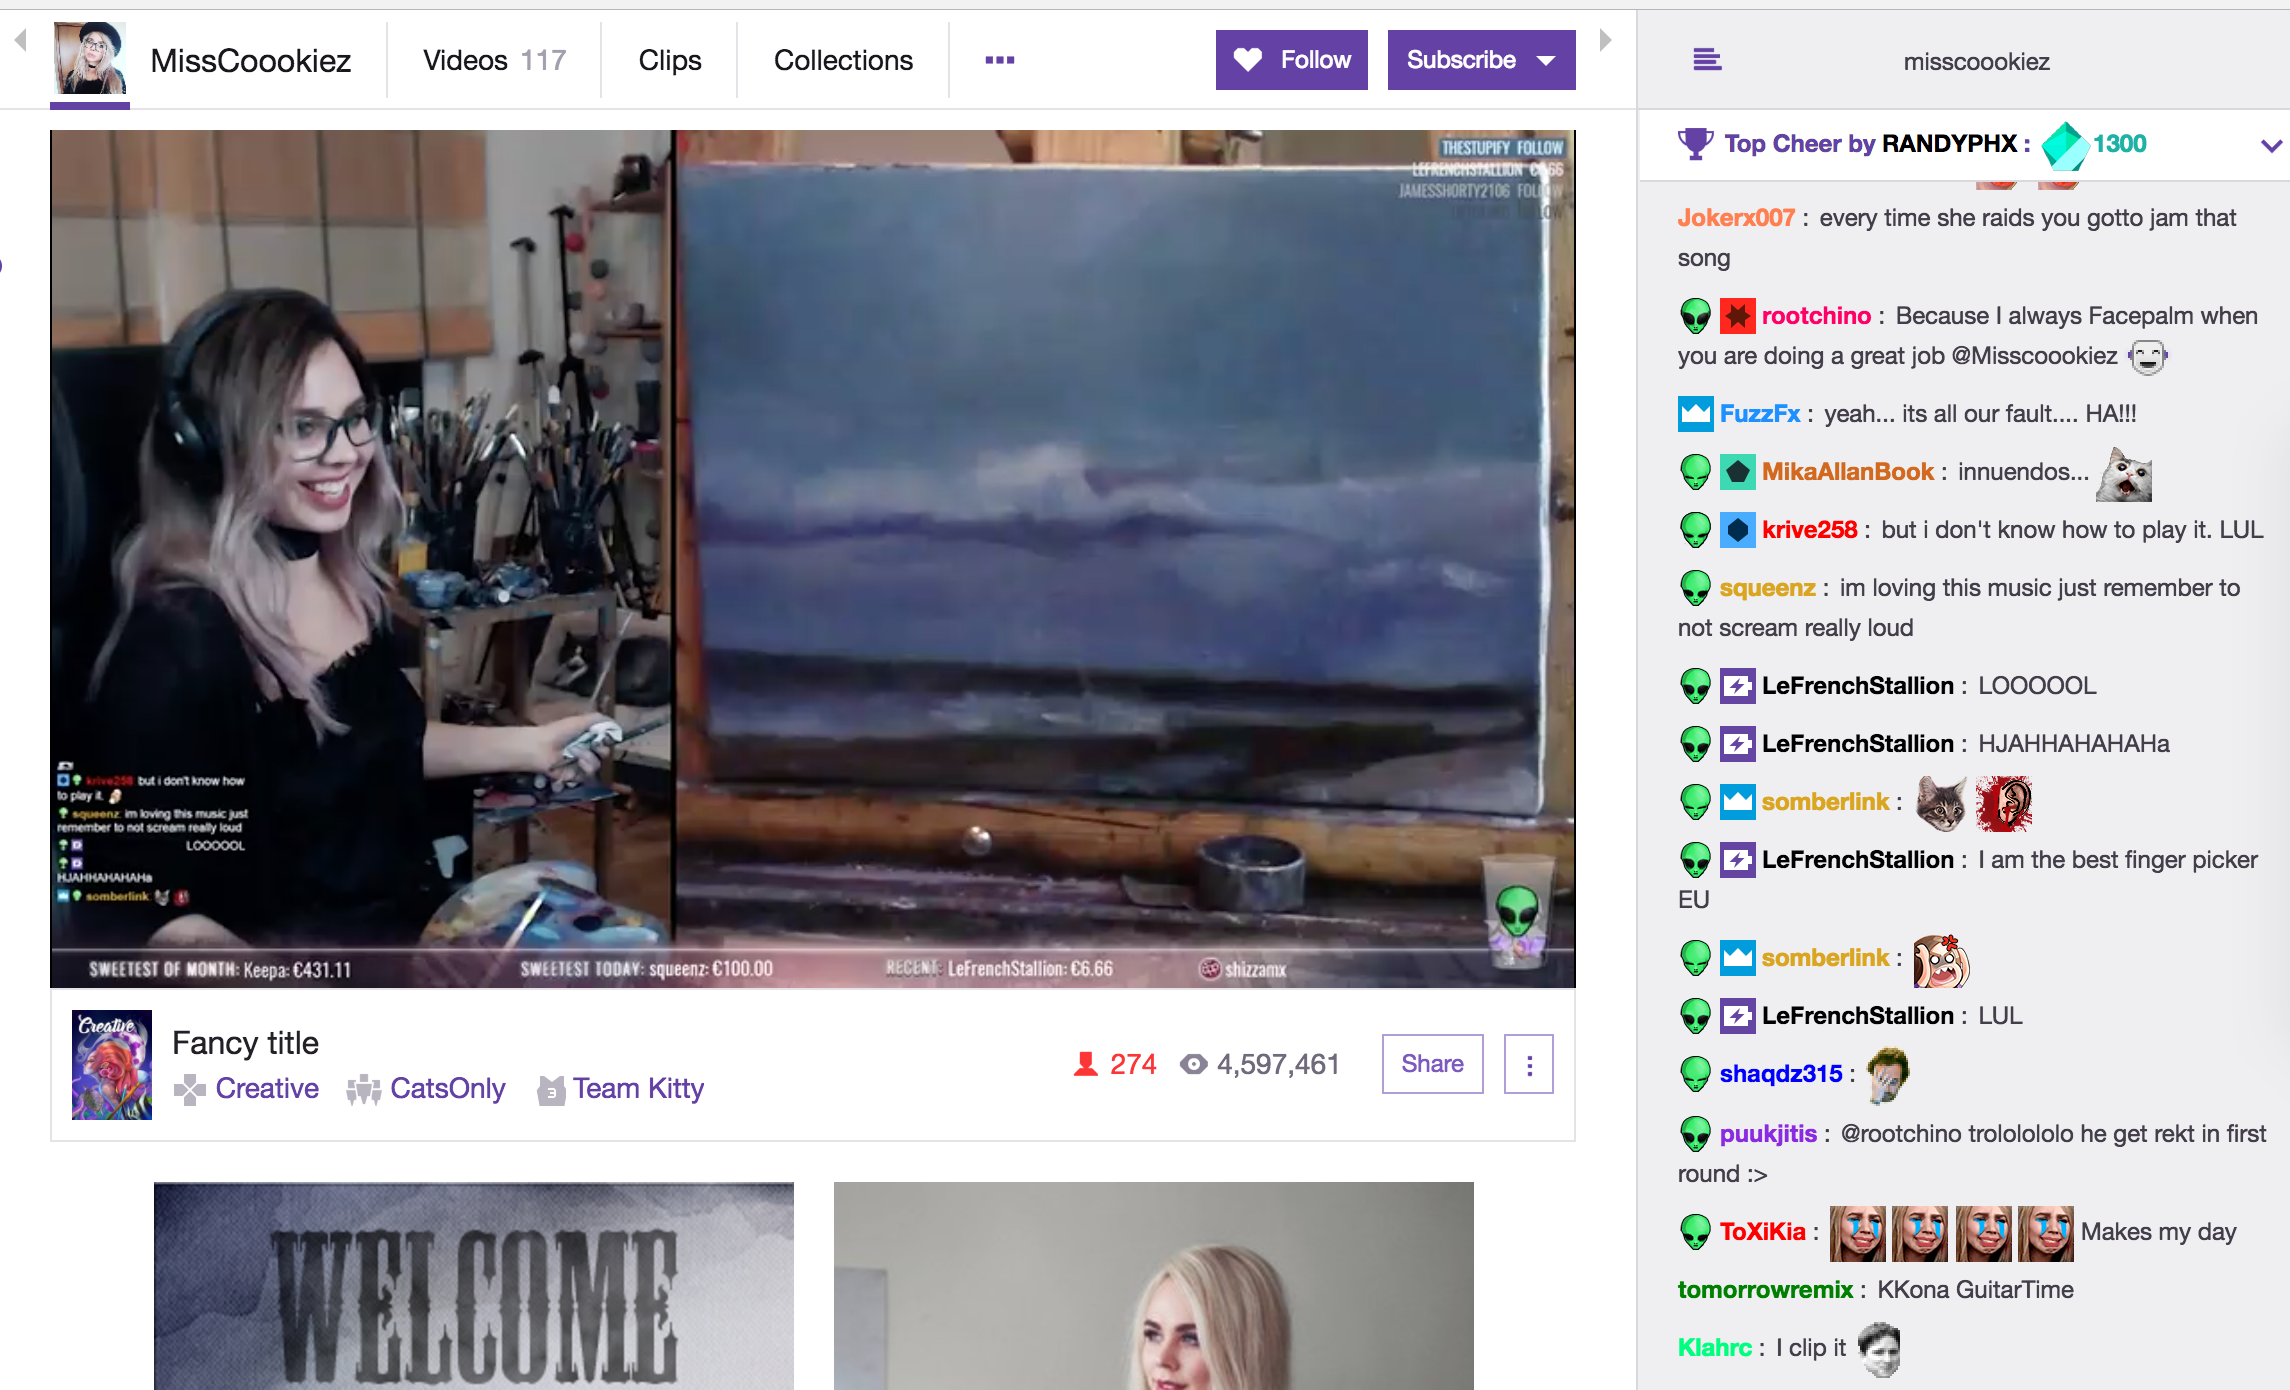
\includegraphics[width=0.5\textwidth]{figures/painting.png}
\caption{\label{fig:Magic}A popular streamer on Twitch painting and talking to her viewers, who chat with her and tip her in real time.}
\end{wrapfigure}
Video sharing sites like YouTube and Twitch
have captured the attention of billions of people around the world
in the span of little more than a decade.
Content producers
--- known informally as ``YouTubers'' and ``streamers'' ---
have begun to make their livings on these sites.
Indeed, these performers have come to rely on
the technical infrastructure these platforms provide as well as
the access to broad audiences and the promise of exposure.
In doing so, these sites have in a real sense democratized media and entertainment industries by
making the avenues to large audiences substantially more accessible.
And thus, in these transformations into Deweyan--style publics~(\cite{dewey2012public,disalvo2009design}), what started as
a recreational hobby
has become a bustling hub for professional artists to
engage with audiences,
practice their craft, and 
hone their skills~(\cite{Hamilton:2014:STF:2611105.2557048,Zhang:2015:CIL:2736084.2736091}).

But recently, tensions between these online performers and the platforms on which they work have shaken
assumptions performers held regarding the nature of the space they're using,
revealing breakdowns in the expectations of these systems~(\cite{doi:10.1177/1461444809342738}).
Performers on now--defunct Vine called (unsuccessfully) to be better compensated~(\cite{vineWantsMoney,vineInsiderMeeting});
YouTubers meanwhile struggle to defend their unconventional performance work~(\cite{h3h3Lawsuit})
and individually and collectively field accusations of misconduct of various forms~(\cite{youtubeDramaResponses}).
These events highlight the politics of an emerging form of expression and art,
and specifically the sometimes controversial nature of the experimentation that performers engage in.

% One issue frustrating this potential research area is that
One issue research in this area must overcome is that
platforms have changed so dramatically in as few as 5 to 10 years that
it can seem as though researchers are trying to navigate through what seem at times like shifting sands.
Scholarship on content creators loses bearing rapidly when
economic factors motivate performers to turn a recreation or a hobby
--- such as video game streaming~(\cite{Hamilton:2014:STF:2611105.2557048}) --- into a career;
the tension between these entertainers experimenting with content remixing and
the holders of the copyright of the source material
(for example, see~(\cite{Hilderbrand48}))
shifts dramatically when
the platform's copyright enforcement mechanisms advance
not just incrementally but substantially~(\cite{kim2012institutionalization}).
And the popularity of candidate field sites can vary chaotically
(see, for example, Vine reaching as many as 200 million active users and
abrupt shutdown less than a year later~(\cite{vineDecline})).

% \section*{Insight}
\textit{Historical analysis}
% Studying contemporary phenomena through an established framing
can be a helpful way of
making sense of contemporary phenomena and informing early fieldwork.
As we found in a recent paper framing crowd work and gig work as a modern instantiation of \textit{piecework},
scholarship from a parallel or similar domain can
provide us some grounding to make sense of what we've seen and offer a framework for making reasonable predictions~(\cite{pieceworkCrowdworkGigwork}).
We believe that a similar approach can be used here to help make sense of online streaming and video performances.

To that end, we can liken some aspects of online performance art on YouTube and Twitch
to street performance and busking,
allowing us to relate ostensibly new phenomena to robust scholarship.
As is the case with street performance,
online performance isn't restricted to classically trained professionals;
instead, performers (both online and in the streets) practice more experimentally,
drawing on candid interactions with their audiences,
which can change from one performance to the next.

This connection has purchase, but it also has gaps,
mostly owing to the unique nature of the internet~(\cite{miller2011understanding}).
For one thing, most video sharing websites keep videos
in perpetuity
--- that is, unless a complaint over copyright infringement is filed, in which case the lifespan of that ``performance'' can be cut short.
The public that congregates around a performer, too, has a similar permanence that offline busking doesn't;
YouTube comments linger for years after they're made, forming in some sense ``networked publics''~(\cite{boyd2007youth}).
We must also account for the different nature of algorithmic enforcement of rules and policies, and
the near--perfect ability of these platforms to redirect revenue and
even an individual audience member's focus in an instant.

We propose to fill in these gaps in our framing of online performance as a modern instantiation of street performance.
How does the \textit{permanence} of digitally archived videos affect people's willingness to experiment with new formats and styles,
and \textit{how can we enable and encourage riskier, potentially more rewarding experimentation}?
How do networked publics influence whether and how performers engage with their audiences,
and \textit{how can we design publics that engage the audience with each other and with the performer}?
How do laws, and the algorithmically instantiated policies, on video sharing and streaming platforms spur or stifle creative remixing?

\section*{Research Plan}
We propose to carry out qualitative research with major online content producers
on video \textit{streaming} sites such as Twitch and Periscope, and video \textit{sharing} sites like YouTube.
Much of this work will consist of ethnographic fieldwork, semi--structured interviews, and
open--ended exploration of the field site as we find parallels and divergences in the domain
of online performance art from street and other emergent formats of performance and entertainment.
A timeline of these phases is outlined here:

\vspace*{5pt}

\noindent\begin{tabular}{p{.5in}|p{5.5in}}
  \textbf{Term} & \textbf{Primary Research Focus} \\
\hline
Q1  & Identifying potential participants and recruiting participants;
      preliminary interviewing and other surveying fieldwork. \\
\hline
Q2  & Performers' \textit{relationships with audiences},
      noting areas of frustration for performers and intervention opportunities, and
      investigating parallel or similar situations that affect street performers. \\
\hline
Q3  & Performers' \textit{relationships with other performers},
      with an eye toward themes such as affiliations or associations of performers representing performers,
      as well as informal supporting relationships. \\
\hline
Q4  & Performers' \textit{relationships with their respective platforms},
      with particular attention to the politics of using an \textit{ostensibly} ``public'' resource,
      and the circumstances that make salient that these platforms are in fact \textit{privately} owned and operated.
\end{tabular}

\vspace*{5pt}

We will recruit between 10 and 30 YouTube and Twitch content producers whose work is primarily content creation on their respective sites
--- in other words, people who have gone ``full--time''.
We will attempt to recruit approximately two--thirds of our participants from YouTube and one--third from Twitch, as
the former is significantly larger (and the community seemingly more diverse), suggesting
a need to get more varied perspectives from participants.

Our interviews will be semi--structured as
we want to be open to the potential for our participants to take us in different directions than originally planned;
nevertheless, we have a bank of interview questions that will
guide the interview along the three major themes we identified earlier:
\begin{inlinelist}
  \item questions about the participant's \textit{relationship with their audiences}
        (e.g. ``do you have personal relationships with other [streamers or YouTubers]?'',
              ``do you think of other [streamers or YouTubers] as `the competition', or potential collaborators, or as something else (or a mix)?'');
  \item questions about the participant's \textit{relationship with other performers}
        (e.g. ``what sorts of comments and feedback do you get?'',
              ``do you respond to comments? change your format or style?''); and
  \item questions about the participant's perceived \textit{relationship with the platform}
        (e.g. ``when did you go `full--time'?'',
              ``what sorts of things get you in trouble on [your platform]?'').
\end{inlinelist}








\pagebreak
\printbibliography{}
\end{document}